\documentclass[handout]{beamer}

\usetheme[progressbar=frametitle]{metropolis}
\metroset{block=fill}

\subtitle{NTIN071 Automata and Grammars}
\author{Jakub Bulín (KTIML MFF UK)}

\date{Spring 2025\\ 
    \vspace{1in} 
    \begin{flushleft}
        \it \footnotesize * Adapted from the Czech-lecture slides by Marta Vomlelová with gratitude. The translation, some modifications, and all errors are mine.
    \end{flushleft}
}

%% packages

\usepackage{amsmath}
\usepackage{amssymb}
\usepackage{amsthm}
\usepackage{cancel}
\usepackage{color}
\usepackage{colortbl}
\usepackage{forest}
\usepackage[utf8x]{inputenc}
\usepackage{multicol}
\usepackage{multirow}

%% colors
\definecolor{Gray}{gray}{0.9}

%% TikZ
\usepackage{tikz}
    \usetikzlibrary{
        automata,
        arrows,
        backgrounds,
        decorations.pathmorphing,
        fit,
        positioning,
        shapes,
        shapes.geometric,
        tikzmark
    } 
    \tikzset{>=stealth',shorten >=1pt,auto,node distance=2cm}
    \tikzset{initial text={}}
    \tikzset{elliptic state/.style={draw,ellipse}}

%% amsthm
\theoremstyle{plain}
    \newtheorem*{algorithm}{Algorithm}    
    \newtheorem*{observation}{Observation}
    \newtheorem*{proposition}{Proposition}

\theoremstyle{remark}
    \newtheorem*{exercise}{Exercise}
    \newtheorem*{remark}{Remark}

%% macros
\DeclareMathOperator{\RegE}{RegE}
\DeclareMathOperator{\RL}{RL}

% Just for Lecture 2
\newcommand{\x}{$\times$}
\newcommand{\nx}{\ }



\title{Lecture 7 -- Pushdown automata}


\begin{document}


\frame{\titlepage}


\begin{frame}{Recap of Lecture 6}
	
    \begin{itemize}
		\item Reducing a grammar: removing $\epsilon$-productions, unit productions, useless symbols
		\item Chomsky Normal Form of a context-free grammar
		\item Pumping lemma for context-free languages, application: proving non-context-freeness
		\item Testing membership in a context-free language: the CYK algorithm
	\end{itemize}
	
\end{frame}


\section{2.9 Pushdown automata}


\begin{frame}{Pushdown automaton (PDA)}

    \vspace{-6pt}
    \begin{center}
        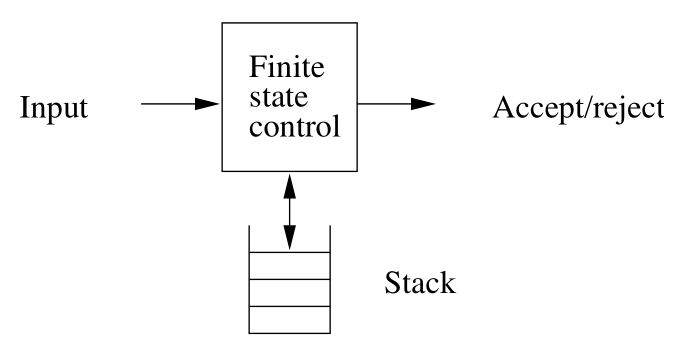
\includegraphics[width=0.6\textwidth]{files/pushDown.PNG}
    \end{center}
    \vspace{-12pt}

    \begin{itemize}
        \item an extension of $\epsilon$--NFA, additional feature: a \alert{stack} memory %(push, pop -- only at the top)
        \item the stack has its own \alert{stack alphabet} $\Gamma$ (can contain $\Sigma$ or not)
        \item at each step we pop the top stack symbol $X$, make a decision based on $(q,a,X)$, push some word $\gamma\in\gamma^*$
        \item the stack can rememeber an infinite amount of information
        \item PDA define context-free languages, nondeterminism is important: \alert{deterministic} PDA only recognize a proper subset of context-free languages (unlike DFA vs. NFA)
    \end{itemize}
    
\end{frame}


\begin{frame}{The definition}

    \alert{A pushdown automaton} (\alert{PDA}): $P=(Q,\Sigma,\Gamma,\delta,q_0,Z_0,F)$, where
        
    \begin{itemize}
        \item $Q$ is finite, nonempty set of states
        \item $\Sigma$ is a finite, nonempty \alert{input alphabet}
        \item $\Gamma$ is a finite, nonempty \alert{stack alphabet}
        \item $\delta$ is the \alert{transition function}, 
        $$
        \delta\colon Q\times (\Sigma\cup \{\epsilon\})\times \Gamma \to \mathcal P_{FIN}(Q \times \Gamma^*)
        $$ 
        $\delta(q,a,X)\ni(p,\gamma)$ where $p$ is the new state and $\gamma$ a finite string of stack symbols that \alert{replace} $X$ on top of the stack
        \item $q_0\in Q$ is the \alert{initial state}
        \item $Z_0\in\Gamma$ is the \alert{initial stack symbol} (\alert{bottom of the stack}); the only symbol on the stack at the beginning
        \item $F$ is a set of \alert{accepting} (\alert{final}) states; may be undefined if our PDA \alert{accepts by empty stack}
    \end{itemize}

\end{frame}


\begin{frame}{One transition of a PDA}   

    \begin{itemize}
        \item read one input letter ($a\in\Sigma$) or do an $\epsilon$-transition ($a=\epsilon$)
        \item pop $X$ from the top of the stack
        \item based on $a$, $X$, and the current state $q$ nondeterministically choose one of finitely many options $(p,\gamma)\in\delta(q,a,X)$
        \item switch to the new state $p$
        \item push the finite string $\gamma$ to the stack (the first symbol of $\Gamma$ is now on top)
        \item \alert{pop}: $\gamma=\epsilon$, \alert{read} only: $\gamma=X$, \alert{push}: $\gamma=\gamma'X$
\end{itemize}

\end{frame}


\begin{frame}{Example: $L_{wwr}=\{ww^R\mid w \in \{0,1\}^*\}$}

    \begin{center}
        \scalebox{0.95}{
        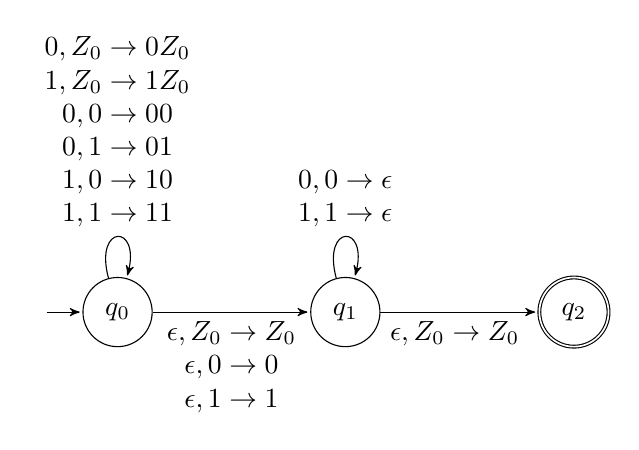
\begin{tikzpicture}[]
            \node[initial,state] (q0)      {$q_0$};
            \node[state] (q1)  [right=2cm of q0]     {$q_1$};
            \node[state, accepting] (q2)  [right=2cm of q1]    {$q_2$};
            \path[->]
                (q0)  edge[loop above]  node[align=center] {
                                        $0,Z_0 \rightarrow 0Z_0$	\\
                                        $1,Z_0 \rightarrow 1Z_0$	\\			
                                        $0,0 \rightarrow 00$	\\			
                                        $0,1 \rightarrow 01$	\\			
                                        $1,0 \rightarrow 10$	\\			
                                        $1,1 \rightarrow 11$			
                                        } (q0)
                (q0)  edge[swap]  node[align=center] {
                                        $\epsilon,Z_0 \rightarrow Z_0$	\\			
                                        $\epsilon,0 \rightarrow 0$	\\			
                                        $\epsilon,1 \rightarrow 1$			
                                        }  (q1)
                (q1)  edge[loop above]  node[align=center] {
                                        $0,0 \rightarrow \epsilon$	\\			
                                        $1,1 \rightarrow \epsilon$			
                                        } (q1)
                (q1)  edge[swap]  node[align=center] {
                                        $\epsilon,Z_0 \rightarrow Z_0$	
                                        } (q2)
                ;
        \end{tikzpicture}
        }
    \end{center}

    \vspace{-12pt}   
    
    \alert{$q_0$} read input letters pushing them onto the stack; guess the middle (nondeterministically), jump to $q_1$\\
    \alert{$q_1$} compare input with stack, consuming both; if empty stack (we see the bottom), accept by jumping to $q_2$; no input can remain

\end{frame}


\begin{frame}{Example cont'd: full description of the PDA}

    \begin{center}
        $P=(\{q_0,q_1,q_2\},\{0,1\},\{0,1,Z_0\},\delta,q_0,Z_0,\{q_2\})$
    \end{center}

    \begin{tabular}{l l}\hline
        $\delta(q_0,0,Z_0)=\{(q_0,0Z_0)\}$ &  
            \multirow{2}{*}{push input onto stack, leave the bottom} \\
        $\delta(q_0,1,Z_0)=\{(q_0,1Z_0)\}$ &  \\\hline
        $\delta(q_0,0,0)=\{(q_0,00)\}$ &  
            \multirow{4}{*}{stay in $q_0$, push input onto stack}\\ 
        $\delta(q_0,0,1)=\{(q_0,01)\}$ \\
        $\delta(q_0,1,0)=\{(q_0,10)\}$ \\
        $\delta(q_0,1,1)=\{(q_0,11)\}$ \\ \hline
        $\delta(q_0,\epsilon,Z_0)=\{(q_1,Z_0)\}$ &
            \multirow{3}{*}{jump to $q_1$ without changing stack}\\ 
        $\delta(q_0,\epsilon,0)=\{(q_1,0)\}$ \\
        $\delta(q_0,\epsilon,1)=\{(q_1,1)\}$ \\ \hline
        $\delta(q_1,0,0)=\{(q_1,\epsilon)\}$ &
            \multirow{2}{*}{pop stack and match with input}\\ 
        $\delta(q_1,1,1)=\{(q_1,\epsilon)\}$ \\ \hline
        $\delta(q_1,\epsilon,Z_0)=\{(q_2,Z_0)\}$ & we have $ww^R$, go to accepting state
        \\\hline
    \end{tabular}

\end{frame}


\begin{frame}{Notation}

    \begin{center}
        \begin{tabular}{l l}
            $a,b,c$ & symbols of the input alphabet\\
            $q,p, r$ & states\\
            $u,w,x,y,z$ & words over input alphabet\\
            $X,Y,A,B$ & stack symbols\\
            $Z_0$ & bottom of the stack symbol\\
            $\alpha,\beta,\gamma$ & words over stack alphabet		
        \end{tabular}
    \end{center}

    \bigskip

    Transition diagram:
    \begin{itemize}
        \item nodes are states, initial and final denoted as usual
        \item a transition $\delta(q,a,X)\ni (p,\alpha)$: arc from $p$ to $q$ labelled $a,X\rightarrow \alpha$          
    \end{itemize}

\end{frame}


\section*{The languages of a PDA}


\begin{frame}{Configurations and moves (computation graph)}

    A \alert{configuration} of a PDA is a triple \alert{$(q,w,\gamma)$}, where
    \begin{description}
        \item[$q$] is the current state 
        \item[$w$] is the remaining input and
        \item[$\gamma$] is the stack contents (the top is on the left) 
    \end{description}

    We define \alert{moves} between configurations (\alert{$\vdash_P$} or \alert{$\vdash$}) thus: for any transition $\delta(q,a,X)\ni(p,\alpha)$ and all $w\in \Sigma^*$ and $\beta\in \Gamma^*$ we have
    $$
    (q,aw,X\beta)\vdash (p,w,\alpha\beta)
    $$
    We use the symbol \alert{$\vdash^*_P$} or \alert{$\vdash^*$} to represent zero or more moves, i.e.
    \begin{itemize}
        \item $I\vdash^*I$ for any configuration $I$
        \item $I\vdash^*J$ if there exists $K$ such that $I\vdash K$ and $K\vdash^*J$
    \end{itemize}

\end{frame}


\begin{frame}{Initial and accepting configurations, the languages of a PDA}

    The \alert{initial configuration} of $P=(Q,\Sigma,\Gamma,\delta,q_0,Z_0,F)$ for input word $w\in\Sigma^*$ is \alert{$(q_0,w,Z_0)$}. Which configurations are \alert{accepting}? 
    
    Two options:

    \textbf{1. Acceptance by final state:} \alert{$(f,\epsilon,\gamma)$} for some final state $f\in F$ and arbitrary stack contents $\gamma\in\Gamma^*$


    $\alert{L(P)}=\{w\mid (q_0,w,Z_0)\vdash^*_P (f,\epsilon,\gamma)\text{ for some }f\in F\text{ and }\gamma\in\Gamma^*\}$

    \bigskip

    \textbf{2. Acceptance by empty stack:} \alert{$(q,\epsilon,\epsilon)$} for an arbitrary $q\in Q$

    $\alert{N(P)}=\{w\mid (q_0,w,Z_0)\vdash^*_P (q,\epsilon,\epsilon)\text{ for any }q\in Q\}$

    \medskip

    In this case we can write only $P=(Q,\Sigma,\Gamma,\delta,q_0,Z_0)$    

\end{frame}


\begin{frame}{Configurations for the input $w=1111$}

    \begin{center}
        \scalebox{0.8}{
            \begin{forest}
                for tree={edge=->}
                [{$(q_0, 1111, Z_0)$},tikz={\node [draw,green,fit=()] {};}
                    [{$(q_0, 111, 1Z_0)$}
                    [{$(q_0, 11, 11Z_0)$}
                    [{$(q_0, 1, 111Z_0)$}
                    [{$(q_0, \epsilon, 1111Z_0)$}[{$(q_1, \epsilon, 1111Z_0)$}]]
                    [{$(q_1, 1, 111Z_0)$}[{$(q_1, \epsilon, 11Z_0)$}]]]
                    [{$(q_1, 11, 11Z_0)$}[{$(q_1, 1, 1Z_0)$}[{$(q_1, \epsilon, Z_0)$}[{$(q_2, \epsilon, Z_0)$},tikz={\node [draw,red,fit=()] {};}]]]]
                    ]
                [{$(q_1, 111, 1Z_0)$}[{$(q_1, 11, Z_0)$}[{$(q_2, 11, Z_0)$}]]]
                ]
                [{$(q_1, 1111, Z_0)$}[{$(q_2, 1111, Z_0)$}]]
                ]
            \end{forest}
        }
    \end{center}

\end{frame}


\begin{frame}{Our example}

    \begin{center}
        \scalebox{0.85}{
        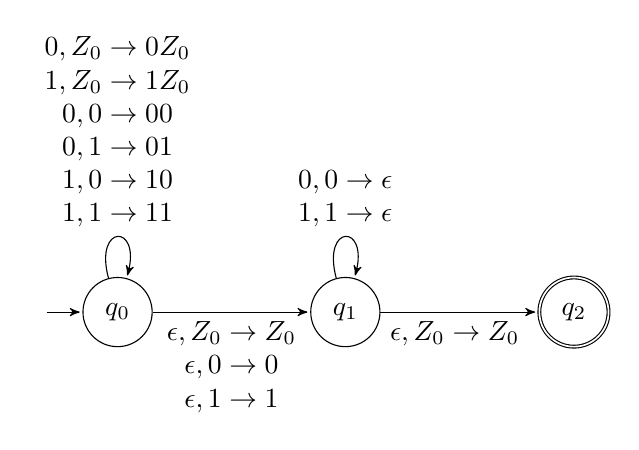
\begin{tikzpicture}[]
            \node[initial,state] (q0)      {$q_0$};
            \node[state] (q1)  [right=2cm of q0]     {$q_1$};
            \node[state, accepting] (q2)  [right=2cm of q1]    {$q_2$};
            \path[->]
                (q0)  edge[loop above]  node[align=center] {
                                        $0,Z_0 \rightarrow 0Z_0$	\\
                                        $1,Z_0 \rightarrow 1Z_0$	\\			
                                        $0,0 \rightarrow 00$	\\			
                                        $0,1 \rightarrow 01$	\\			
                                        $1,0 \rightarrow 10$	\\			
                                        $1,1 \rightarrow 11$			
                                        } (q0)
                (q0)  edge[swap]  node[align=center] {
                                        $\epsilon,Z_0 \rightarrow Z_0$	\\			
                                        $\epsilon,0 \rightarrow 0$	\\			
                                        $\epsilon,1 \rightarrow 1$			
                                        }  (q1)
                (q1)  edge[loop above]  node[align=center] {
                                        $0,0 \rightarrow \epsilon$	\\			
                                        $1,1 \rightarrow \epsilon$			
                                        } (q1)
                (q1)  edge[swap]  node[align=center] {
                                        $\epsilon,Z_0 \rightarrow \alert{Z_0}$	
                                        } (q2)
                ;
        \end{tikzpicture}
        }
    \end{center}

    \begin{itemize}
        \item acceptance by final state: $L(P)=L_{wwr}$
        \item to accept by empty stack: modify $\delta(q_1,\epsilon,Z_0)=\{(q_2,Z_0)\}$ to $\delta(q_1,\epsilon,Z_0)=\{(q_2,\epsilon)\}$ (erase bottom of the stack symbol), then also $N(P')=L_{wwr}$
    \end{itemize}

\end{frame}


\begin{frame}{Another example: if-else}

    Stop (accept) at first error, e.g. more $\mathtt{else}$'s than $\mathtt{if}$'s

    \textbf{By empty stack:} {\small $P_N=(\{q\},\{\mathtt{if},\mathtt{else}\},\{Z\},\delta_N,q,Z)$}

    \begin{columns}

        \small

        \column{0.48\textwidth}

        \begin{center}
            \scalebox{0.87}{
                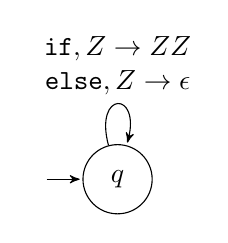
\begin{tikzpicture}
                    \node[initial,state] (q) {$q$};
                    \path[->]
                        (q)  edge[loop above] node[align=center] { $\mathtt{if},Z\rightarrow ZZ$\\ $\mathtt{else},Z\rightarrow \epsilon$} (q);
                \end{tikzpicture}
            }
        \end{center} 

        \column{0.52\textwidth}

        \begin{itemize}
            \item[] $\delta_N(q,\mathtt{if},Z)=\{(q,ZZ)\}$ \hfill(push)
            \item[] $\delta_N(q,\mathtt{else},Z)=\{(q,\epsilon)\}$ \hfill(pop)
        \end{itemize}
        
    \end{columns}

    \medskip

    \textbf{By final state:} {\small $P_F=(\{p,q,r\},\{\mathtt{if},\mathtt{else}\},\{Z,X_0\},\delta_F,p,X_0,\{r\})$}

    \begin{columns}

        \small

        \column{0.48\textwidth}

        \begin{center}
            \scalebox{0.87}{
                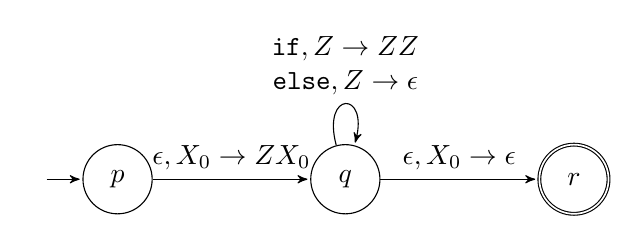
\begin{tikzpicture}
                    \node[initial,state] (p)      {$p$};
                    \node[state] (q) [right=2cm of p]     {$q$};
                    \node[state,accepting] (r) [right=2cm  of q]     {$r$};
                    \path[->]
                        (q)  edge[loop above] node[align=center] { $\mathtt{if},Z\rightarrow ZZ$\\ $\mathtt{else},Z\rightarrow \epsilon$} (q)
                        (p)  edge node {$\epsilon,X_0\rightarrow ZX_0$} (q)
                        (q)  edge node {$\epsilon,X_0\rightarrow \epsilon$} (r);
                \end{tikzpicture}
            }
        \end{center}          
        
        \column{0.52\textwidth}
        
        \begin{itemize}
            \item[] $\delta_F(p,\epsilon,X_0)=\{(q,ZX_0)\}$ \hfill (start)
            \item[] $\delta_F(q,\mathtt{if},Z)=\{(q,ZZ)\}$ \hfill (push)
            \item[] $\delta_F(q,\mathtt{else},Z)=\{(q,\epsilon)\}$ \hfill (pop)
            \item[] $\delta_F(q,\epsilon,X_0)=\{(r,\epsilon)\}$ \hfill (accept)
        \end{itemize}
        
    \end{columns}

\end{frame}


\begin{frame}{From empty stack to final state}

    \begin{lemma}
        If $L=N(P_N)$ for some PDA $P_N=(Q,\Sigma,\Gamma,\delta_N,q_0,Z_0)$, then there is a PDA $P_F$ such that $L=L(P_F)$.
    \end{lemma}

    \begin{center}
        \scalebox{0.9}{
            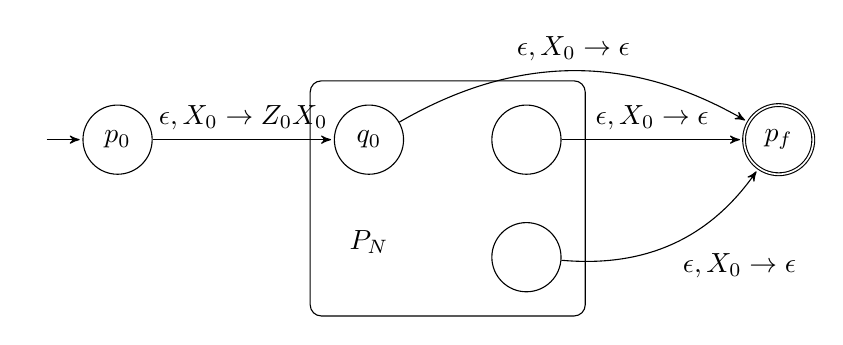
\begin{tikzpicture}
                \node[initial,state] (p0)      {$p_0$};
                \node[state] (q0)  [right=2.3cm of p0]    {$q_0$};
                \node[state] (q1a)   [right of=q0]   {};
                \node[state] (q1b)   [below=.6cm of q1a]   {};
                \node[state,draw=none] (pf) [below=.4cm of q0] {$P_N$};
                \node[state,accepting] (q2)   [right=2.3cm of q1a] {$p_f$};
                \node[state] (X)[rectangle,  fit= (q0) (q1a) (q1b), inner sep=0.3cm,rounded corners] {};
                \path[->]
                    (p0)  edge node {$\epsilon,X_0 \rightarrow Z_0X_0$} (q0)
                    (q0)  edge[bend left] node {$\epsilon, X_0\rightarrow \epsilon$} (q2)
                    (q1a)  edge node {$\epsilon, X_0\rightarrow \epsilon$} (q2)
                    (q1b)  edge[bend right] node[swap] {$\epsilon,X_0\rightarrow \epsilon$} (q2);        
            \end{tikzpicture}
        }
    \end{center}

    \textbf{Idea:} Make $Z_0$ a fake bottom (insert a new bottom $X_0$ below), so that we can tell when $P_N$'s stack was empty. Add $\epsilon$-transitions upon seeing $X_0$ from all states to a new, accepting state.

\end{frame}


\begin{frame}{The proof}

    $P_F=(Q\cup \{p_0,p_f\},\Sigma,\Gamma\cup\{X_0\},\delta_F,p_0,X_0,\{p_F\})$, where $\delta_F$ is
    \begin{itemize}
        \item $\delta_F(p_0,\epsilon,X_0)=\{(q_0,Z_0X_0)\}$ (start).
        \item $\forall (q\in Q, a\in \Sigma\cup\{\epsilon\},Y\in \Gamma)$, $\delta_F(q,a,Y)=\delta_N(q,a,Y)$.
        \item In addition, $\delta_F(q,\epsilon,X_0)\ni (p_f,\epsilon)$ for every $q\in Q$.
    \end{itemize}
    We must show that $w\in L(P_N)$ iff $w\in L(P_F)$.
    \begin{itemize}
        \item (If) $P_F$ accepts as follows: $(p_0,w,X_0)\vdash_{P_F}(q_0,w,Z_0X_0)\vdash^*_{P_F=N_F}(q,\epsilon,X_0)\vdash_{P_F}(p_f,\epsilon,\epsilon) $.
        \item (Only if) No other way to go to $p_F$ than the above. \hfill\qedsymbol
    \end{itemize}
    

\end{frame}


\begin{frame}{From final state to empty stack}

    \begin{lemma}
        If $L=L(P_F)$ for some PDA  
        $P_F=(Q,\Sigma,\Gamma,\delta_F,q_0,Z_0,F)$, then there exists a PDA $P_N$ such that $L=N(P_N)$.
    \end{lemma} 
    
    \begin{center}
        \scalebox{0.95}{
            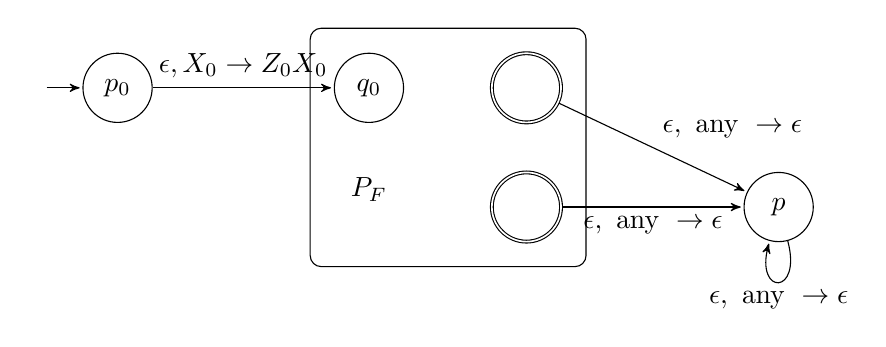
\begin{tikzpicture}
                \node[initial,state] (p0)      {$p_0$};
                \node[state] (q0)  [right=2.3cm of p0]    {$q_0$};
                \node[state,accepting] (q1a)   [right of=q0]   {};
                \node[state,accepting] (q1b)   [below=.6cm of q1a]  {};
                \node[state,draw=none] (pf) [below=.4cm of q0] {$P_F$};
                \node[state] (q2)   [right=2.3cm of q1b] {$p$};
                \node[state] (X)[rectangle,  fit= (q0) (q1a) (q1b), inner sep=0.3cm,rounded corners] {};
                \path[->]
                    (p0)  edge node {$\epsilon,X_0 \rightarrow Z_0X_0$} (q0)
                    (q1a)  edge node {$\epsilon, \hbox{ any }\rightarrow \epsilon$} (q2)
                    (q1b)  edge node[swap] {$\epsilon,\hbox{ any }\rightarrow \epsilon$} (q2)
                    (q2)  edge[loop below] node {$\epsilon,\hbox{ any }\rightarrow\epsilon$} (q2);
            \end{tikzpicture}            
        }
    \end{center}
    \vspace{-12pt}

    \textbf{Idea:} Make $Z_0$ a fake bottom (insert a new bottom below), because $P_F$ could accidentally empty stack in a nonfinal state. Add $\epsilon$-transitions (upon any stack symbol) from final states to a new state, there empty the stack without reading any input symbols.

\end{frame}


\begin{frame}{The proof}

    Let $P_N=(Q\cup \{p_0,p\},\Sigma,\Gamma\cup\{X_0\},\delta_N,p_0,X_0)$, where
    \begin{itemize}
        \item $\delta_N(p_0,\epsilon,X_0)=\{(q,Z_0X_0)\}$ (start)
        \item $\forall (q\in Q, a \in \Sigma\cup\{\epsilon\},Y\in \Gamma)$ $\delta_N(q,a,Y)=\delta_F(q,a,Y)$ (simulate)
        \item $\forall (q \in F,Y\in \Gamma\cup\{X_0\})$, $\delta_N(q,\epsilon,Y)\ni (p,\epsilon)$ (i.e. accept if $P_F$ accepts)
        \item $\forall (Y\in \Gamma\cup\{X_0\}), \delta_N(p,\epsilon,Y)=\{ (p,\epsilon)\}$ clean the stack.
    \end{itemize}
    The proof $w\in N(P_N)$ iff $w\in L(P_F)$ is similar as before.\hfill\qedsymbol

\end{frame}


\begin{frame}{Unseen data cannot affect computation}

    \begin{lemma}
        If $(q,x,\alpha)\vdash_P (p,y,\beta) $, then for any $w\in \Sigma^*$ and $\gamma\in\Gamma^*$ we also have 
        $(q,xw,\alpha\gamma)\vdash^*_P(p,yw,\beta\gamma)$. (In particular, $\gamma=\epsilon$ or $w=\epsilon$.)
    \end{lemma}
    \textbf{Proof:} Induction on the number length of the sequence of configurations that take $(q,xw,\alpha\gamma)$ to $(p,yw,\beta\gamma)$. Each of the moves $(q,x,\alpha)\vdash^*_P(p,y,\beta)$ is justified without using $w$ and/or $\gamma$ in any way. The moves are still valid with $w,\gamma$ on the input/stack.\hfill\qedsymbol

    \medskip

    \begin{lemma}
        If $(q,xw,\alpha)\vdash^*_P (p,yw,\beta) $, then also $(q,x,\alpha)\vdash^*_P(p,y,\beta)$.
    \end{lemma}
    \textbf{NB:} Not true for stack, the computation may require $\gamma$ on the stack and then push it back. (E.g. $L=\{0^i1^i0^j1^j\}$, configuration $(p,0^{i-j}1^i0^j1^j,0^jZ_0)\vdash^* (q,1^j,0^jZ_0)$, inbetween clear the stack.)

\end{frame}


\section*{2.10 Equivalence of PDA and context-free grammars}


\begin{frame}{Equivalence of PDA and CFG}

    \begin{theorem}
        The following statements about $L\subset\Sigma^*$ are equivalent:
        \begin{enumerate}[(i)]
            \item There exists a context-free grammar such that $L(G)=L$.
            \item There exists a PDA such that $L(P)=L$.
            \item There exists a PDA such that $N(P)=L$.
        \end{enumerate}
    \end{theorem}
        
    \begin{center}
        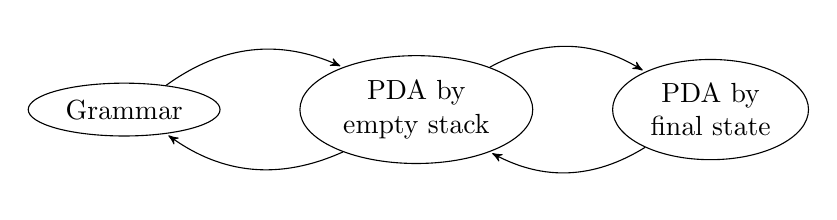
\begin{tikzpicture}
            \node[elliptic state] (p)      {Grammar};
            \node[elliptic state][align=center] (q) [right=1cm of p]     {PDA by\\empty stack};
            \node[elliptic state][align=center] (r) [right=1cm  of q]     {PDA by\\final state};
            \path[->]
                (p)  edge[bend left] node {} (q)
                (q)  edge[bend left] node {} (p)
                (q)  edge[bend left] node {} (r)
                (r)  edge[bend left] node {} (q)
            ;
        \end{tikzpicture}    
    \end{center}

    We have already shown $(ii)\Leftrightarrow(iii)$. To prove equivalence with a context-free grammar, we use acceptance by empty stack.

\end{frame}


\section*{Context-free grammar to pushdown automaton}


\begin{frame}{CFG to PDA}

    \begin{block}{The construction}
        Given $G=(V,T,\mathcal P,S)$, construct $P=(\{q\},T,V\cup T,\delta,q,S)$:
        \begin{enumerate}[(1)]
            \item for each $ A\in V$, \alert{$\delta(q,\epsilon, A)=\{(q,\beta)\mid A\rightarrow \beta \in\mathcal P\}$} \\ \hfill [apply rule]
            \item for each $a\in T$, \alert{$\delta(q,a,a)=\{(q,\epsilon)\}$}\\ \hfill [match terminal]
        \end{enumerate}   
    \end{block} 

    \textbf{How it works:}
    \begin{itemize}
        \item a \alert{leftmost} derivation is simulated by the PDA
        \item current sentential form = part of input read + stack contents
        \item see a variable: apply rule, a terminal: read \& pop from stack
    \end{itemize}

\end{frame}


\begin{frame}{An example}

    \begin{example}
        $I\rightarrow a\mid b\mid Ia\mid Ib\mid I0\mid I1$,\\
        $E\rightarrow I\mid E*E\mid E+E\mid (E)$
    \end{example}
        
    $\Sigma=\{a,b,0,1,(,),+,*\}$, $\Gamma=\Sigma\cup\{I,E\}$,  $\delta$ is defined as follows:

    \begin{itemize}
        \item $\delta(q,\epsilon,I)=\{(q,a),(q,b),(q,Ia),(q,Ib),(q,I0),(q,I1)\}$
        \item $\delta(q,\epsilon,E)=\{(q,I),(q,E*E),(q,E+E),(q,(E))\}$
        \item $\delta(q,s,s)=\{(q,\epsilon)\}$ for all $s\in \Sigma$ (e.g. $\delta(q,+,+)=\{(q,\epsilon)\}$)
        \item $\delta(q,x)$ is empty otherwise
    \end{itemize}

    \alert{Leftmost derivation:} $E\Rightarrow E*E\Rightarrow I*E\Rightarrow a*E\Rightarrow a*I\Rightarrow a*b$\\       	
    
    \medskip

    The sequence of configurations:

    $(q,a*b,E)$
    $\vdash$ $(q,a*b,E*E)$
    $\vdash$ $(q,a*b,I*E)$
    $\vdash$ $(q,a*b,a*E)$
    $\vdash$ $(q,*b,*E)$
    $\vdash$ $(q,b,E)$
    $\vdash$ $(q,b,I)$
    $\vdash$ $(q,b,b)$
    $\vdash$ $(q,\epsilon,\epsilon)$

\end{frame}


\begin{frame}{The proof that $N(P)=L(G)$\hfill \alert{(i) $w\in L(G)\Rightarrow w\in N(P)$}}

    Start with a leftmost derivation $S=\gamma_1\Rightarrow_{lm}\ldots\Rightarrow_{lm}\gamma_n=w$.

    Prove by induction on $i$ that $(q,w,S)\vdash_P^* (q, v_i,\alpha_i)$, where $\gamma_i=u_i\alpha_i$ is the $i$-th sentential form and $u_iv_i=w$.

    If $\gamma_i$ contains only terminals, set $\gamma_i=w=u_i, v_i=\epsilon=\alpha_i$. Otherwise, write $\gamma_i=u_iA\alpha_i$, where $u_i\in T^*$ and $A\in V$ is the leftmost variable.

    By induction we have $(q,w,S)\vdash_P^* (q, v_i,A\alpha_i)$, $w=u_iv_i$.

    For the step $\gamma_i\Rightarrow_{lm}\gamma_{i+1}$ we used some rule $A\rightarrow\beta\in P$. The PDA replaces $A$ on the stack with $\beta$, moves to configuration $(q,v_i,\beta\alpha_i)$.

    We pop all terminals $v\in \Sigma^*$ from the beginning of $\beta\alpha$ (matching them with the input): $v_i=vv_{i+1}$ and $\beta\alpha=v\alpha_{i+1}$

    We got to $(q,v_{i+1},\alpha_{i+1})$, corresponds to the sentential form $\gamma_{i+1}$.
    
\end{frame}


\begin{frame}{The proof that $N(P)=L(G)$\hfill \alert{(ii) $w\in N(P)\Rightarrow w\in L(G)$}}

    \vspace{-3pt}
    Prove that if $(q,u,X)\vdash_P^*(q,\epsilon,\epsilon)$, then $X\Rightarrow_G^* u$. By induction on the number of moves. \textbf{Basis} \alert{$n=1$} move:
    \begin{itemize}
        \item $X=a\in\Sigma$: $\delta(q, a, a)\ni (q,\epsilon)$, $u=a$, 0-step derivation
        \item $X=A\in \Gamma$: $\delta(q,\epsilon,A)\ni (q,\epsilon)$ coming from $A\rightarrow\epsilon\in\mathcal P$, $u=\epsilon$
    \end{itemize} 

    \vspace{-3pt}
    \textbf{Induction step} \alert{$n>1$} moves: if the first move is \alert{[match terminal]}, don't extend the derivation, if it is \alert{[apply rule]}: $A$ on top of stack was replaced by $\beta=Y_1Y_2\ldots Y_k$, for a rule $A\to\beta\in\mathcal P$.

    \begin{columns}

        \column{0.78\textwidth}
    
        Split $u=u_1\ldots u_k$ s.t. while popping $Y_i$ we read~$u_i$, i.e. $(q,u_iu_{i+1}\ldots u_k,Y_i)\vdash^*(q,u_{i+1}\ldots u_k,\epsilon)$

        \medskip
        
        Thus also $(q,u_i,Y_i)\vdash^*(q,\epsilon,\epsilon)$, by induction assumption we get $Y_i\Rightarrow^*u_i$. Together:
        {\small
        $$
        A\Rightarrow Y_1Y_2\ldots Y_k\Rightarrow^* u_1Y_2\ldots Y_k\Rightarrow^* \ldots \Rightarrow^* u_1u_2\ldots u_k
        $$
        } 
        
        \vspace{-6pt}\hfill\qedsymbol
    
        \column{0.22\textwidth}

        \scalebox{0.85}{
            \input{files/PDACFG.pdf_t}
        }
        
    \end{columns}    
       
\end{frame}


\end{document}


\section*{Pushdown automaton to context-free grammar}





\begin{frame}{PDA to CFG: an example}

    \begin{columns}

        \column{0.7\textwidth}\centering
        
        Given $P=(\{q\},\{\mathtt{if},\mathtt{else}\},\{Z\},\delta,q,Z)$
        
        \smallskip

        $\delta(q,\mathtt{if},Z)=\{(q,ZZ)\}$\\        
        $\delta(q,\mathtt{else},Z)=\{(q,\epsilon)\}$
        
        \column{0.3\textwidth}

        \begin{center}
            \scalebox{0.9}{
                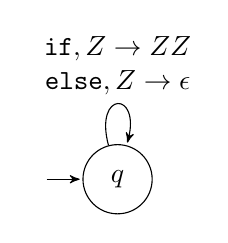
\begin{tikzpicture}
                    \node[initial,state] (q) {$q$};
                    \path[->]
                        (q)  edge[loop above] node[align=center] { $\mathtt{if},Z\rightarrow ZZ$\\ $\mathtt{else},Z\rightarrow \epsilon$} (q);
                \end{tikzpicture}
            }
        \end{center} 

    \end{columns}

    Construct $G=(V,\{\mathtt{if},\mathtt{else}\},\mathcal P,S)$

    \begin{itemize}
        \item variables: $V=\{S,[qZq]\}$ 
        {\small
        \hfill\alert{$V=\{S\}\cup\{[pXq]\mid p,q\in Q,X\in\Gamma\}$}\\
        \hfill\alert{$[pXq]$ $\sim$ go from $p$ to $q$, pop $X$}
        }
        \item production rules:
        \begin{itemize}
            \item $S\rightarrow [qZq]$
            {\small\hfill\alert{$S\to [q_0Xr]$ for $r\in Q$}\\
            \item $[qZq]\rightarrow \mathtt{else}$
            \item $[qZq]\rightarrow \mathtt{if}[qZq][qZq]$
        \end{itemize}
        \item in this example, $S$ and $[qZq]$ generate the same words, so we can simplify:
         $G=(\{S\},\{\mathtt{if},\mathtt{else}\},\{S\rightarrow \mathtt{if}SS\mid\mathtt{else}\},S)$
        
    \end{itemize}      
    
\end{frame}


\end{document}


    \begin{columns}[c] 
    \column{0.8\textwidth} 
    \begin{example}
    Převeďme PDA $P_N=(\{q\},\{i,e\},\{Z\},\delta_N,q,Z)$ na obrázku na gramatiku.
    \begin{itemize}[<+->]
        \item Neterminály gramatiky budou $V=\{S,[qZq]\}$ nový start a jediná trojice $P_N$.
        \item Pravidla:
            \begin{itemize}
            \item $S\rightarrow [qZq]$.
            \item $[qZq]\rightarrow e$
            \item $[qZq]\rightarrow i[qZq][qZq]$.
        \end{itemize}
        Můžeme nahradit trojici $[qZq]$ symbolem $A$ a dostaneme:
        $S\rightarrow A$\\
        $A\rightarrow iAA|e$.\\
        Protože $A$ a $S$ odvozují přesně stejné řetězce, můžeme je ztotožnit:
        $G=(\{S\},\{i,e\},\{S\rightarrow iSS|e\},S)$.
    \end{itemize}
    \end{example}
    \column{0.19\textwidth} 
        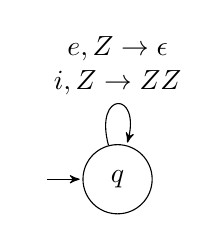
\begin{tikzpicture}
                \node[initial,state] (q)      {$q$};
    %			\node[state,accepting] (q1) [right of=q0]     {};
            \path[->]
                    (q)  edge[loop above] node[align=center] {$e,Z\rightarrow\epsilon$\\ $i,Z\rightarrow ZZ$} (q)
                    ;
            \end{tikzpicture}
    \end{columns}
    
    \end{frame}




\begin{itemize}
	\item The key event: PDA pops one symbol off the stack. The state before and after the popping may be different.
\item Grammar variables are composite symbols $[qXr_k]$, $q,r_k\in Q, X\in \Gamma$
\item we add new starting variable $S$.
\end{itemize}

\begin{example}
\begin{multicols}{2}
Let us convert the PDA $$P_N=(\{q\},\{i,e\},\{Z\},\delta_N,q,Z)$$ (see the figure on the right) to a grammar.


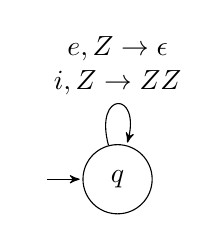
\begin{tikzpicture}
			\node[initial,state] (q)      {$q$};
%			\node[state,accepting] (q1) [right of=q0]     {};
		\path[->]
				(q)  edge[loop above] node[align=center] {$e,Z\rightarrow\epsilon$\\ $i,Z\rightarrow ZZ$} (q)
				;
		\end{tikzpicture}
\end{multicols}

\begin{itemize}
	\item Grammar variables are $V=\{S,[qZq]\}$ the new start and the only triple from $P_N$.
	\item Production:
		\begin{itemize}
		\item $S\rightarrow [qZq]$.
		\item $[qZq]\rightarrow i[qZq][qZq]$.
		\item $[qZq]\rightarrow e$
	\end{itemize}
	We may replace the triple $[qZq]$ by the symbol $A$ and we get:
	$S\rightarrow A$\\
	$A\rightarrow iAA\mid e$.\\
	If we notice that $A$ and $S$ derive exactly the same strings, we identify them as one, and we get:
	$G=(\{S\},\{i,e\},\{S\rightarrow iSS\mid e\},S)$.
\end{itemize}

\end{example}

\bigskip

\begin{theorem}[Grammar for a PDA]
Let $P=(Q,\Sigma,\Gamma,\delta,q_0,Z_0)$ be a PDA. Then there is a context-free grammar $G$ such that $L(G)=N(P)$.
\end{theorem}

Productions will be:
\begin{itemize}
	\item $\forall p_\ell \in Q$: $S\rightarrow [q_0Z_0p_\ell]$, i.e. guess the end state $p_\ell$ and run the PDA to $(q_0,w,Z_0)\vdash^*(p_\ell,\epsilon,\epsilon)$.
\item For all pairs $(r,Y_1Y_2\ldots Y_k)$ in all $\delta(q,a,X)$, all $r_i \in Q$, create a production
$$[qXr_k]\rightarrow a[rY_1r_1][r_1Y_2r_2]\ldots [r_{k-1}Y_kr_k]\hbox{.}
$$
\item In particular, for $(r,\epsilon)\in\delta(q,a,A)$ add the production rule $[qAr]\to a$.
\end{itemize}

\begin{proof}
The proof that:
$[qXp]\Rightarrow^*w\hbox{ if and only if} (q,w,X)\vdash^*(p,\epsilon,\epsilon)
$
is done in both directions by induction (number of moves, number of steps in the derivation.)
\end{proof}		

\begin{example}[$\{0^n1^n; n>0\}$]{\,}

\begin{multicols}{2}
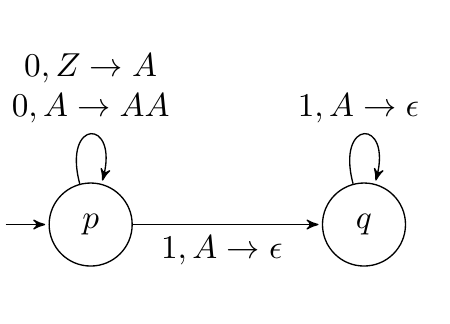
\begin{tikzpicture}[]
\useasboundingbox (-0.8,-0.9) rectangle (4.2,2.5);
    \scope[transform canvas={scale=1.2}]
			\node[initial,state] (p)      {$p$};
			\node[state] (q)  [right=2cm of p]     {$q$};
		\path[->]
				(p)  edge[loop above]  node[align=center] {
								$0,Z \rightarrow A$	\\
								$0,A \rightarrow AA$	
								} (p)
				(p)  edge[swap]  node[align=center] {
								$1,A \rightarrow \epsilon$			
								}  (q)
				(q)  edge[loop above]  node[align=center] {
								$1,A \rightarrow \epsilon$			
								} (q)
				;
    \endscope
\end{tikzpicture}

\columnbreak

\begin{tabular}{l l c}
$\delta$ & Productions & \\\hline
& $S\rightarrow [pZp]\mid [pZq]$ & (1)\\
								$\delta(p,0,Z)\ni (p,A)$	& $[pZp]\rightarrow 0[pAp] $ & (2)\\
									& $[pZq]\rightarrow 0[pAq] $& (3)\\
								$\delta(p,0,A)\ni (p,AA)$ & $[pAp]\rightarrow 0[pAp][pAp] $& (4)	\\
								 & $[pAp]\rightarrow 0[pAq][qAp] $	& (5)\\
								 & $[pAq]\rightarrow 0[pAp][pAq] $& (6)	\\
								 & $[pAq]\rightarrow 0[pAq][qAq] $	& (7)\\
								$\delta(p,1,A)\ni (q,\epsilon)$ & $[pAq]\rightarrow 1 $ & (8)\\			
								$\delta(q,1,A)\ni (q, \epsilon)$ & $[qAq]\rightarrow 1 $& (9)			
\end{tabular}

\end{multicols}

Derivation of $0011$:
$S\Rightarrow^{(1)} [pZq] \Rightarrow^{(3)} 0[pAq]\Rightarrow^{(7)} 00[pAq][qAq]\Rightarrow^{(8)} 001[qAq]\Rightarrow^{(9)} 0011$
\end{example}




\begin{frame}{Příklad: Od zásobníkového automatu ke gramatice}
    %\begin{proof}
    %Pro $w\in \Sigma^*$ dokazujeme\\
    %$[qXp]\Rightarrow^* w \hbox{ právě když } (q,w,X)\vdash^*(p,\epsilon,\epsilon)
    %$\\
    %indukcí v obou směrech (počet kroků PDA, počet kroků derivace.)
    %\end{proof}
    \begin{columns}[c] 
    \column{0.8\textwidth} 
    \begin{example}
    Převeďme PDA $P_N=(\{q\},\{i,e\},\{Z\},\delta_N,q,Z)$ na obrázku na gramatiku.
    \begin{itemize}[<+->]
        \item Neterminály gramatiky budou $V=\{S,[qZq]\}$ nový start a jediná trojice $P_N$.
        \item Pravidla:
            \begin{itemize}
            \item $S\rightarrow [qZq]$.
            \item $[qZq]\rightarrow e$
            \item $[qZq]\rightarrow i[qZq][qZq]$.
        \end{itemize}
        Můžeme nahradit trojici $[qZq]$ symbolem $A$ a dostaneme:
        $S\rightarrow A$\\
        $A\rightarrow iAA|e$.\\
        Protože $A$ a $S$ odvozují přesně stejné řetězce, můžeme je ztotožnit:
        $G=(\{S\},\{i,e\},\{S\rightarrow iSS|e\},S)$.
    \end{itemize}
    \end{example}
    \column{0.19\textwidth} 
        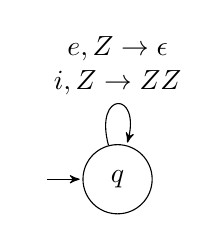
\begin{tikzpicture}
                \node[initial,state] (q)      {$q$};
    %			\node[state,accepting] (q1) [right of=q0]     {};
            \path[->]
                    (q)  edge[loop above] node[align=center] {$e,Z\rightarrow\epsilon$\\ $i,Z\rightarrow ZZ$} (q)
                    ;
            \end{tikzpicture}
    \end{columns}
    
    \end{frame}
    %\begin{frame}{Ekvivalence jazyků rozpoznávaných zásobníkovými automaty a bezkontextových jazyků}
    
    \begin{frame}{Od zásobníkového automatu ke gramatice CFG}
    \begin{columns}[c] 
    \column{0.74\textwidth} 
    \begin{itemize}[<+->] 
        \item Zásobní automat bere \alert{jeden} symbol ze zásobníku. Stav před a po kroku může být různý.
    \item Neterminály gramatiky budou složené symboly $[qXp]$, PDA vyšel z $q$, vzal $X$ a přešel do $p$; 
    \begin{itemize}
        \item[] a zavedeme nový počáteční symbol $S$.
    \end{itemize}
    %\item Na obrázku $[p_0Y_1p_1],[p_1Y_2p_2],\ldots,[p_{k-1}Y_kp_k]$.
    \end{itemize}
    \pause
    \begin{lemmaN}[Gramatika pro PDA]\label{lem:LG}
    Mějme PDA $P=(Q,\Sigma,\Gamma,\delta,q_0,Z_0)$. Pak existuje bezkontextová gramatika $G$ taková, že $L(G)=N(P)$.
    \end{lemmaN}
    \column{0.25\textwidth} 
    \input{PDACFG2.pdf_t}
    \end{columns}
    Pravidla definujeme:
    \begin{itemize}[<+->]
        \item $\forall p \in Q$: $S\rightarrow [q_0Z_0p]$, tj. uhodni koncový stav a spusť PDA na $(q_0,w,Z_0)\vdash^*(p,\epsilon,\epsilon)$.
    \item Pro všechny dvojice $({\color{red}p},Y_1Y_2\ldots Y_k)\in\delta({\color{red}q,s,X}), s\in \Sigma \cup \{\epsilon\}, \forall p_1,\ldots,p_{k-1} \in Q$ vytvoř pravidlo
    $$[{\color{red}qX}{\color{blue}p_k}]\rightarrow {\color{red}s}[{\color{red}p}Y_1p_1][p_1Y_2p_2]\ldots [p_{k-1}Y_k{\color{blue}p_k}]
    $$
    \item spec. pro $(p,\epsilon)\in\delta(q,a,A)$ vytvoř $[qAp]\rightarrow a$.
    \end{itemize}
    \end{frame}
    
    
    %\begin{theorem*}
    %Následující tvrzení jsou ekvivalentní
    %\begin{itemize}
        %\item Jazyk $L$ je bezkontextový, tj. generovaný CFG
        %\item Jazyk $L$ je přijímaný nějakým zásobníkovým automatem koncovým stavem.
        %\item Jazyk $L$ je přijímaný nějakým zásobníkovým automatem prázdným zásobníkem.
    %\end{itemize}
    %\end{theorem*}
        %\begin{tikzpicture}
                %\node[elliptic state][align=center] (p)      {bezkontextová\\ gramatika};
                %\node[elliptic state][align=center] (q) [right=1cm of p]     {PDA \\ prázdným\\ zásobníkem};
                %\node[elliptic state][align=center] (r) [right=1cm  of q]     {PDA\\ koncovým\\  stavem};
            %\path[->]
                    %(p)  edge[bend left] node {} (q)
                    %(q)  edge[bend left] node {} (p)
                    %(q)  edge[bend left] node {} (r)
                    %(r)  edge[bend left] node {} (q)
                    %;
            %\end{tikzpicture}
    %
    %\end{frame}
    %
    %\begin{frame}{Od zásobníkového automatu ke gramatice CFG}
    %\begin{columns}[c] 
    %\column{0.74\textwidth} 
    %\begin{itemize}
        %\item Zásobní automat bere \alert{jeden} symbol ze zásobníku. Stav před a po kroku může být různý.
    %\item Neterminály gramatiky budou složené symboly $[pXq]$, PDA vyšel z $p$, vzal $X$ a přešel do $q$; 
    %\begin{itemize}
        %\item[] a zavedeme nový počáteční symbol $S$.
    %\end{itemize}
    %\item Na obrázku $[p_0Y_1p_1],[p_1Y_2p_2],\ldots,[p_{k-1}Y_kp_k]$.
    %\end{itemize}
    %\begin{theorem}[Gramatika pro PDA]
    %Mějme PDA $P=(Q,\Sigma,\Gamma,\delta,q_0,Z_0)$. Pak existuje bezkontextová gramatika $G$ taková, že $L(G)=N(P)$.
    %\end{theorem}
    %\column{0.255\textwidth} 
      %\begin{center}
        %\includegraphics[width=\textwidth]{C:/Users/marta/Desktop/automaty/pdaPop2.PNG}
      %\end{center}
    %\end{columns}
    %Pravidla definujeme:
    %\begin{itemize}
        %\item $\forall p \in Q$: $S\rightarrow [q_0Z_0p]$, tj. uhodni koncový stav a spusť PDA na $(q_0,w,Z_0)\vdash^*(p,\epsilon,\epsilon)$.
    %\item Pro všechny dvojice $(r,Y_1Y_2\ldots Y_k)\in\delta(q,s,X), s\in \Sigma \cup \{\epsilon\}$ vytvoř pravidlo
    %$$[qXr_k]\rightarrow s[rY_1r_1][r_1Y_2r_2]\ldots [r_{k-1}Y_kr_k]\hbox{.}
    %$$
    %\end{itemize}
    %\end{frame}
    \begin{frame}{}
    \begin{proof}
    Pro $w\in \Sigma^*$ dokazujeme\\
    $[qXp]\Rightarrow^* w$ právě když $ (q,w,X)\vdash^*(p,\epsilon,\epsilon)
    $\\
    indukcí v obou směrech (počet kroků PDA, počet kroků derivace.)
    \end{proof}
    %\begin{columns}[c] 
    %\column{0.8\textwidth} 
    %\begin{example}
    %Převeďme PDA $P_N=(\{q\},\{i,e\},\{Z\},\delta_N,q,Z)$ na obrázku na gramatiku.
    %\begin{itemize}
        %\item Neterminály gramatiky budou $V=\{S,[qZq]\}$ nový start a jediná trojice $P_N$.
        %\item Pravidla:
            %\begin{itemize}
            %\item $S\rightarrow [qZq]$.
            %\item $[qZq]\rightarrow i[qZq][qZq]$.
            %\item $[qZq]\rightarrow e$
        %\end{itemize}
        %Můžeme nahradit trojici $[qZq]$ symbolem $A$ a dostaneme:
        %$S\rightarrow A$\\
        %$A\rightarrow iAA|e$.\\
        %Protože $A$ a $S$ odvozují přesně stejné řetězce, můžeme je ztotožnit:
        %$G=(\{S\},\{i,e\},\{S\rightarrow iSS|e\},S)$.
    %\end{itemize}
    %\end{example}
    %\column{0.19\textwidth} 
        %\begin{tikzpicture}
                %\node[initial,state] (q)      {$q$};
    %%			\node[state,accepting] (q1) [right of=q0]     {};
            %\path[->]
                    %(q)  edge[loop above] node[align=center] {$e,Z\rightarrow\epsilon$\\ $i,Z\rightarrow ZZ$} (q)
                    %;
            %\end{tikzpicture}
    %\end{columns}
    %
    %\end{frame}
    %
    %\begin{frame}{}
    %\begin{proof}
    %The proof that:
    %$[qXp]\Rightarrow^* \hbox{if and only if} (q,w,X)\vdash^*(p,\epsilon,\epsilon)
    %$
    %is done in both direction by induction (number of moves, number of steps in the derivation.)
    %\end{proof}
    \begin{minipage}{\textwidth}
    \begin{minipage}{0.67\textwidth}
    \begin{example}[$\{0^n1^n; n>0\}$]
    \begin{tabular}{l l c}
    $\delta$ & Pravidla & \\\hline
    & $S\rightarrow [pZ_{0}p]|[pZ_{0}q]$ & (1)\\
                                    $\delta(p,0,Z_{0})\ni (p,A)$	& $[pZ_{0}p]\rightarrow 0[pAp] $ & (2)\\
                                        & $[pZ_{0}q]\rightarrow 0[pAq] $& (3)\\
                            $\delta(p,0,A)\ni (p,AA)$ & $[pAp]\rightarrow 0[pAp][pAp] $& (4)	\\
                                     & $[pAp]\rightarrow 0[pAq][qAp] $	& (5)\\
                                     & $[pAq]\rightarrow 0[pAp][pAq] $& (6)	\\
                                     & $[pAq]\rightarrow 0[pAq][qAq] $	& (7)\\
                                    $\delta(p,1,A)\ni (q,\epsilon)$ & $[pAq]\rightarrow 1 $ & (8)\\			
                                    $\delta(q,1,A)\ni (q, \epsilon)$ & $[qAq]\rightarrow 1 $& (9)			
    \end{tabular}
    \end{example}
    \end{minipage}
    \begin{minipage}{0.1092\textwidth}
    \end{minipage}
    \begin{minipage}{0.21\textwidth}
    \begin{tikzpicture}[]
    \useasboundingbox (-0.8,-0.9) rectangle (4.2,2.5);
        \scope[transform canvas={scale=.7}]
                \node[initial,state] (p)      {$p$};
                \node[state] (q)  [right=2cm of p]     {$q$};
            \path[->]
                    (p)  edge[loop above]  node[align=center] {
                                    $0,Z_{0} \rightarrow A$	\\
                                    $0,A \rightarrow AA$	
                                    } (p)
                    (p)  edge[swap]  node[align=center] {
                                    $1,A \rightarrow \epsilon$			
                                    }  (q)
                    (q)  edge[loop above]  node[align=center] {
                                    $1,A \rightarrow \epsilon$			
                                    } (q)
                    ;
        \endscope
            \end{tikzpicture}
    %}
    \end{minipage}
    \end{minipage}
    Derivace $0011$\\
    $S\Rightarrow^{(1)} [pZ_{0}q] \Rightarrow^{(3)} 0[pAq]\Rightarrow^{(7)} 00[pAq][qAq]\Rightarrow^{(8)} 001[qAq]\Rightarrow^{(9)} 0011$
    \end{frame}
    
    \begin{frame}{Shrnutí}
    \begin{itemize}
        \item Zásobníkový automat PDA je $\epsilon$--NFA automat rozšířený o zásobník, potenciálně nekonečnou paměť
        
        \begin{itemize}
            \item a zásobníkovou abecedu, počáteční zásobníkový symbol, přechodová funkce čte a píše na zásobník, píše i řetězec
        \end{itemize}
        \item Přijímání koncovým stavem a prázdným zásobníkem, pro nedeterministiké PDA přijímají stejnou třídu jazyků
        \item a to bezkontextové jazyky, generované bezkontextovými gramatikami.
    \end{itemize}
    \end{frame}
    
    